\section{Modelling the Garland}

Since we assumed that the tree is a cone and that the garland spirals evenly spaced around this cone, we can model the garland as a \emph{circular conical spiral}, and applying lower and upper bounds, it has the parametric function \autocite{rejbrandConicalHelix}:
\begin{equation}
    C(t) = \begin{pmatrix}[0.7]
        at\cos{t} \\
        at\sin{t} \\
        bt
    \end{pmatrix}, \quad \forall t \in \left[0, \frac{H}{b}\right]
\end{equation}
where the constants $a, b \in \Real$. Lower and upper bounds are applied because the cone has height $H$, and as such we only want parts of the curve where $z(t)$ is between $0$ and $H$. Thus, $0 \leq bt \leq H$, and dividing by $b$, we find that $0 \leq t \leq \frac{H}{b}$, which are the bounds that we apply to $C(t)$. $t$ is the independent variable, and for any given value of $t$, the parametric function outputs a point in 3D space. As we generate an infinite amount of points from the lower bound to the upper bound, the locus of points formed results in the shape of the space curve. The z-axis of the spiral coincides with the tree's axis of radial symmetry and $C(0)$ represents the tip of the tree.

\begin{figure}[H]
    \centering
    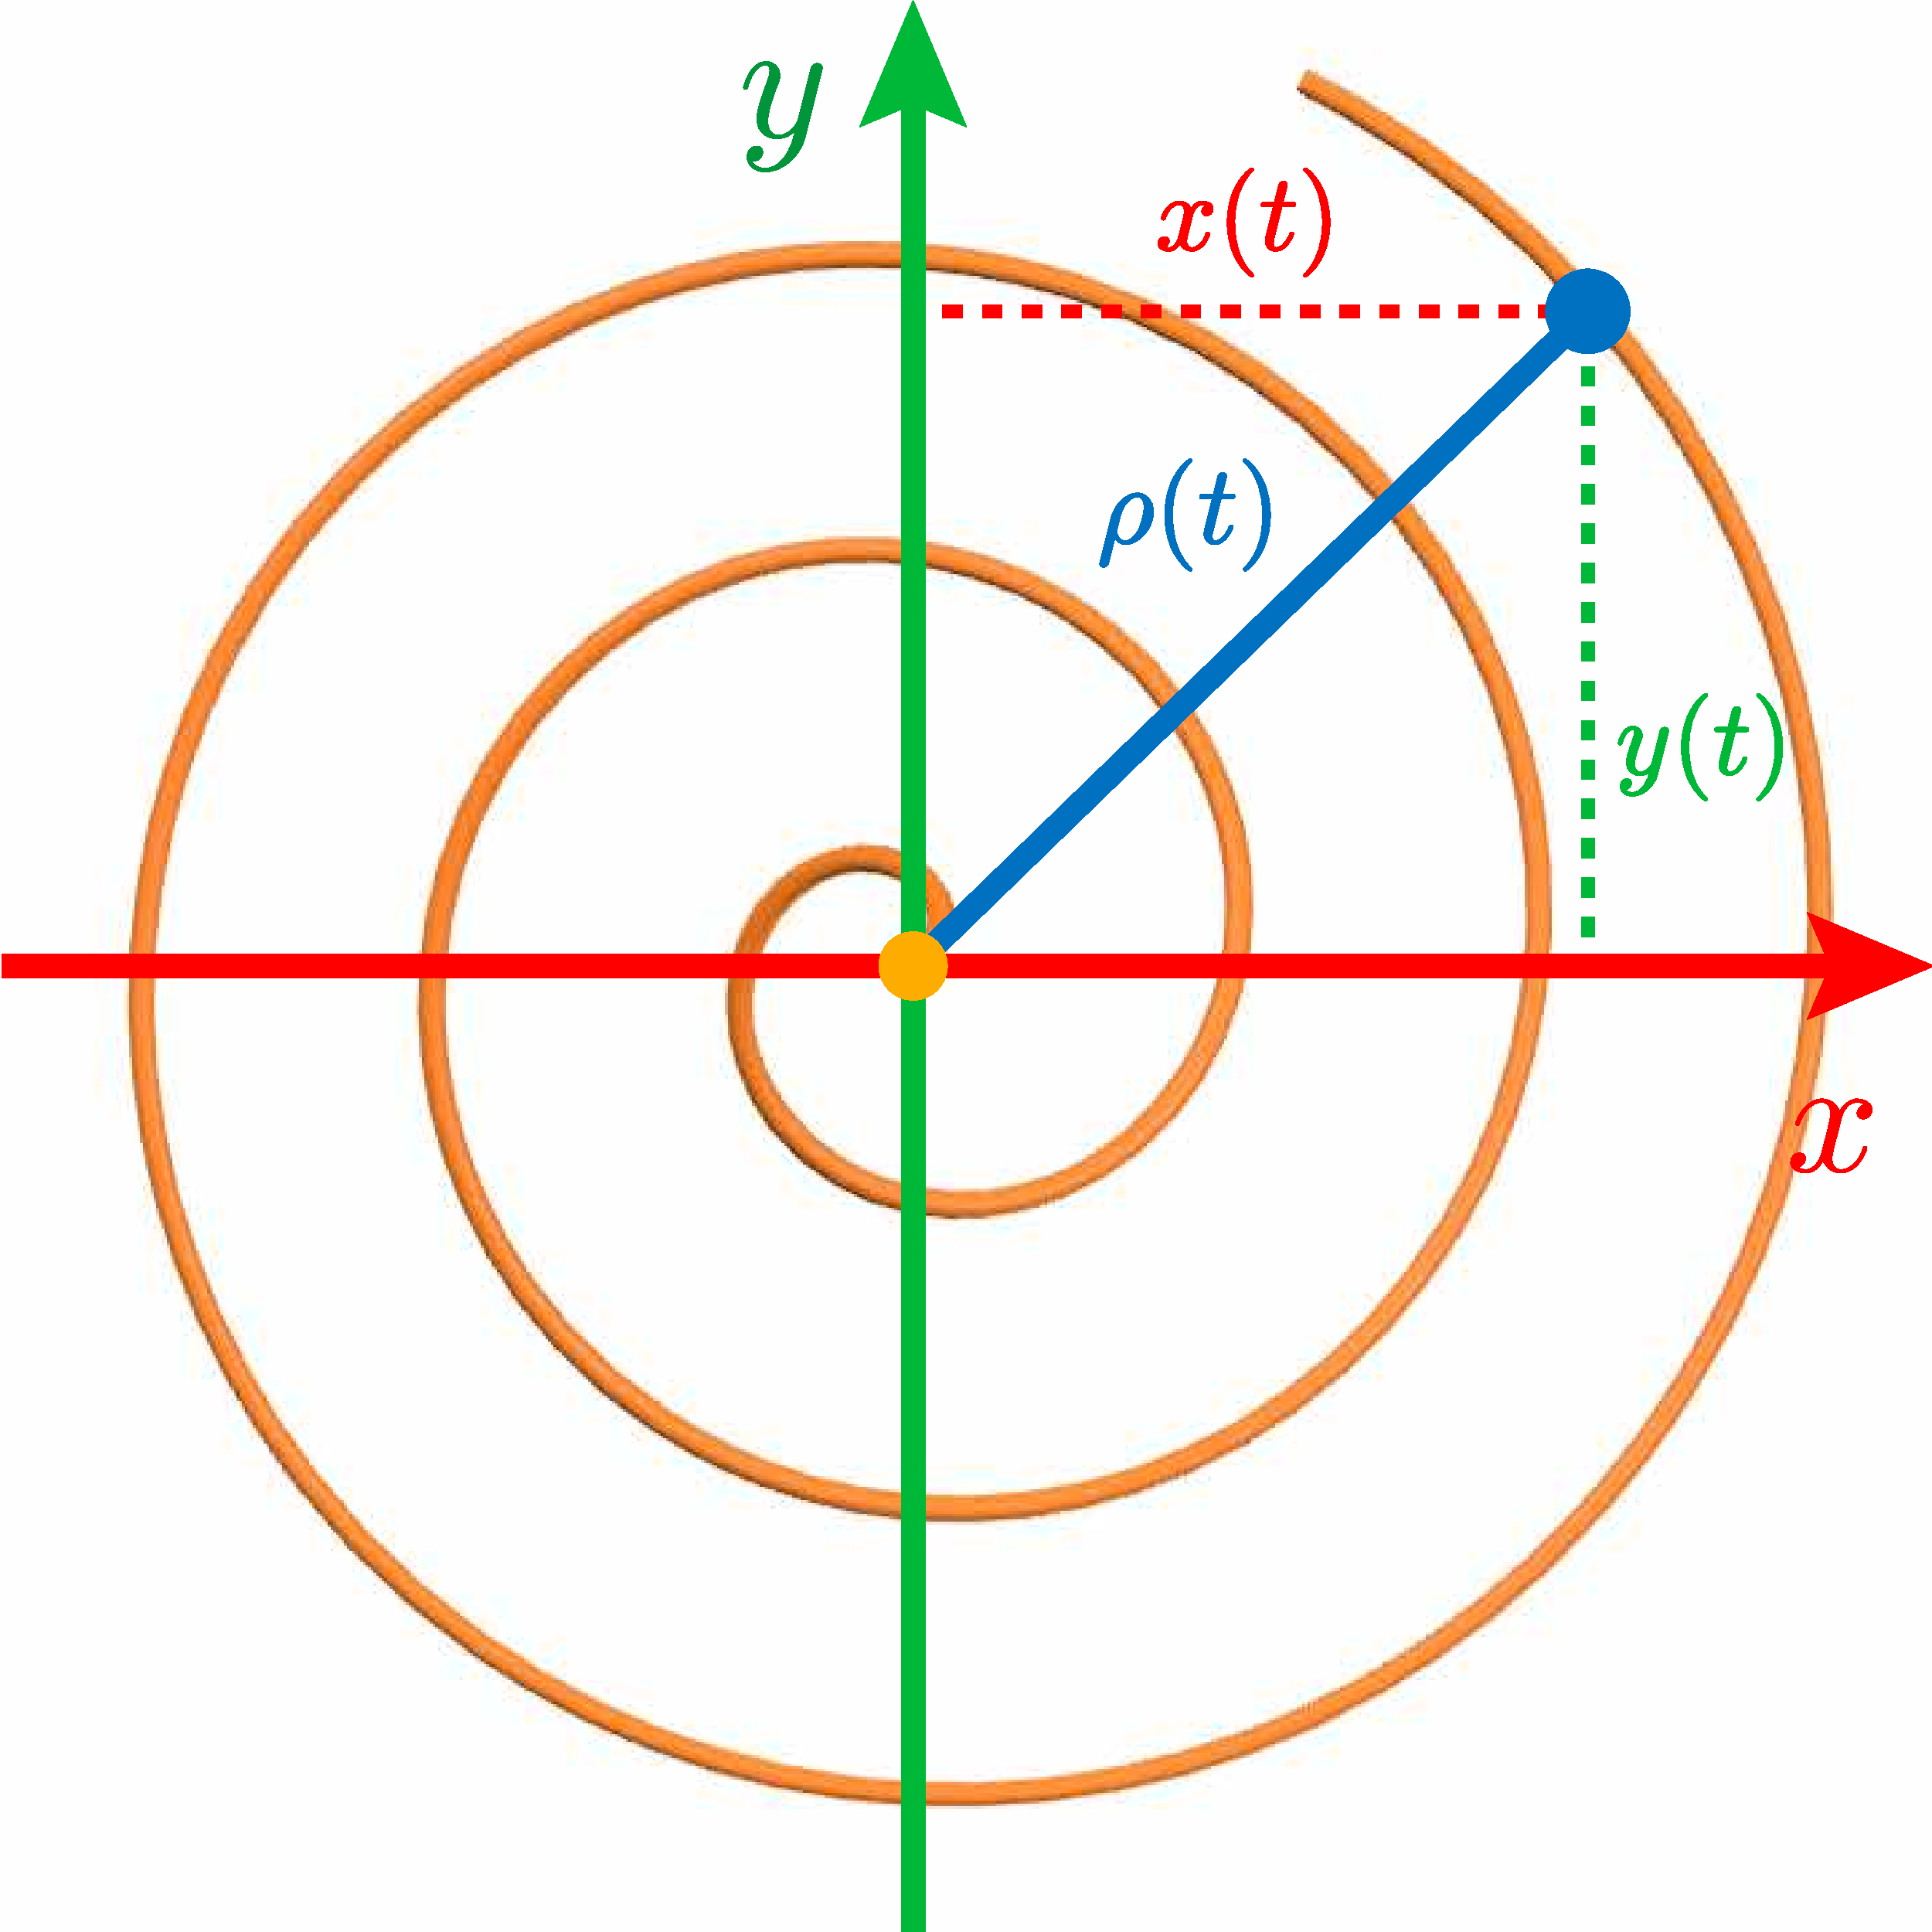
\includegraphics[width=0.42\textwidth]{diagrams/radial_distance.pdf}
    \caption{Radial distance of a point on the spiral to the z-axis (top-down view).} \label{fig:radial}
    \vspace*{-15pt}
\end{figure}

To ensure that the spiral sits on the surface of the cone (the Christmas tree), it is necessary to find appropriate values for $a$ and $b$. Using methodology inspired by a blog post authored by \citeauthor{stewartGarland2014}, we first define the radial distance $\rho(t)$ as the distance of a point on the curve to the tree's axis of radial symmetry, visualized in Figure \ref{fig:radial}. By the Pythagorean theorem:
\begin{equation*}
    \rho(t) = \sqrt{x(t)^2+y(t)^2}
\end{equation*}
\bulletarrow{Substituting for $x(t)$ and $y(t)$:}
\begin{align}
    \rho(t) & = \sqrt{a^2t^2\cos^2{t}+a^2t^2\sin^2{t}} \notag \\
            & = at\sqrt{\cos^2{t}+\sin^2{t}} \notag           \\
            & = at
\end{align}

\clearpage
\begin{wrapfigure}{l}{0.32\textwidth}
    \centering
    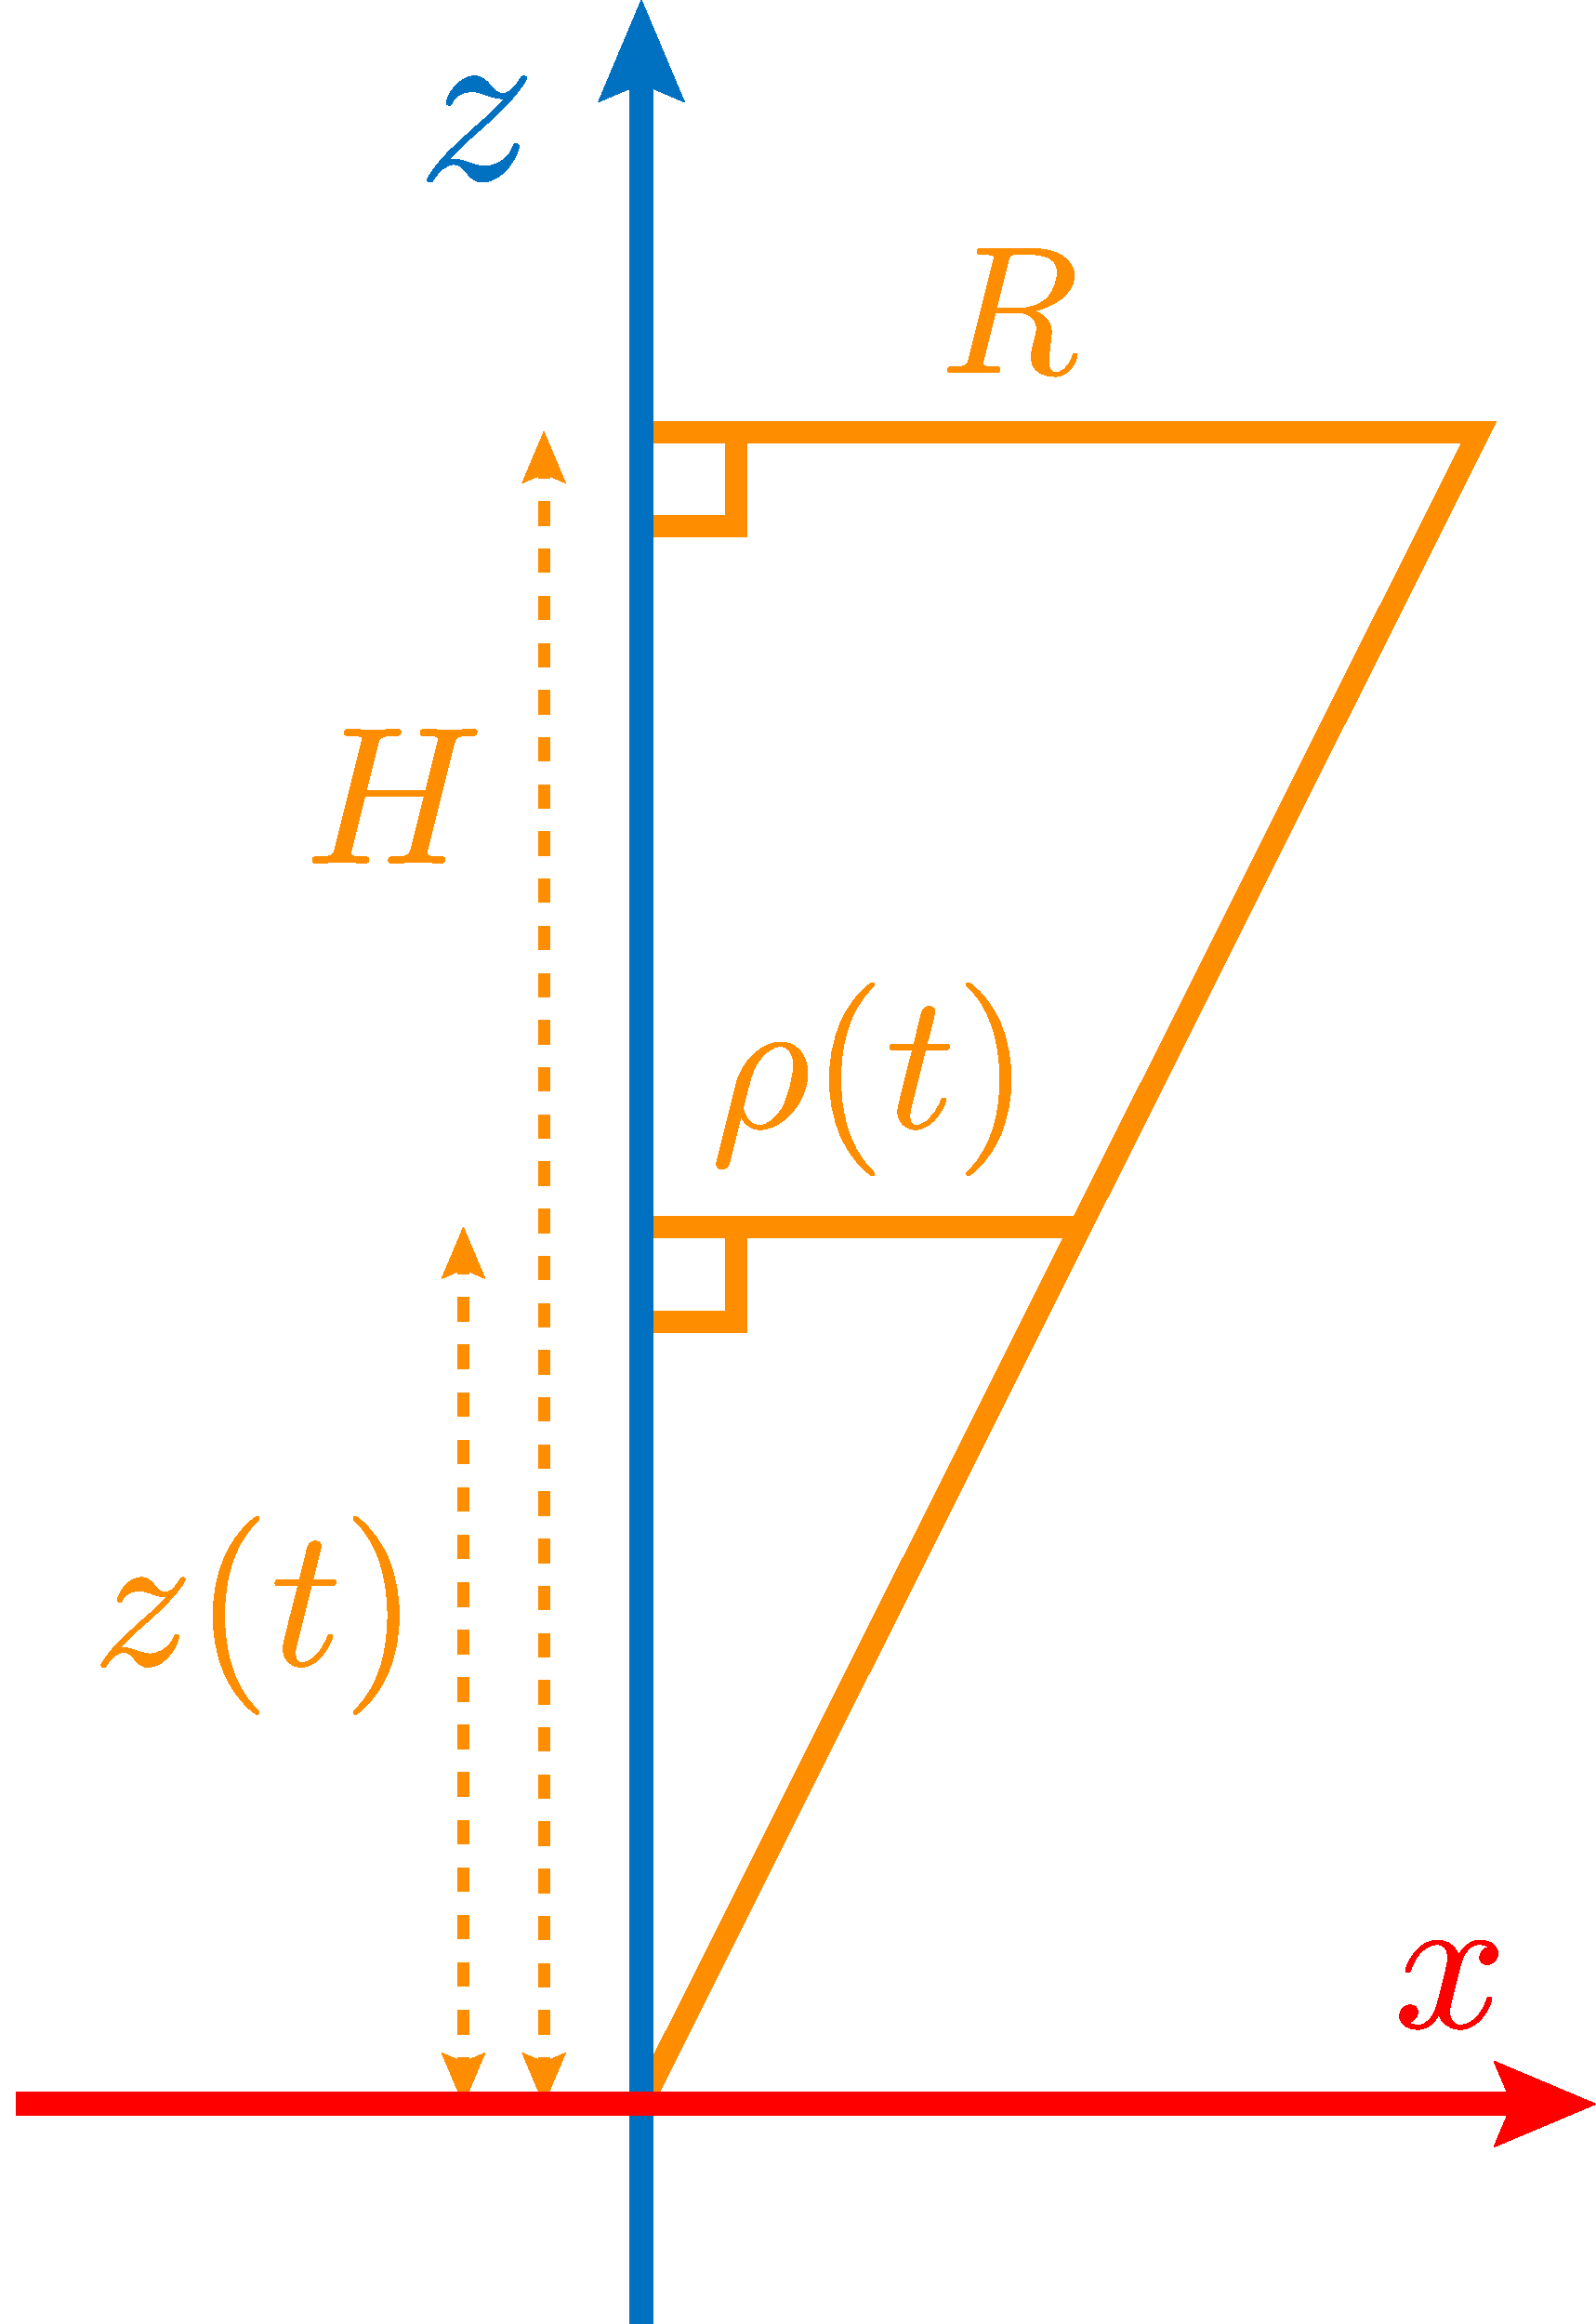
\includegraphics[width=0.3\textwidth]{diagrams/similar_triangles.pdf}
    \caption{Similar Triangles.} \label{fig:sim_tri}
\end{wrapfigure}
The radial distance is useful because any valid point of the curve should sit on the surface of the cone of height $H$ and radius $R$, and thus the right triangle with base lengths equal to the radial distance $\rho(t)$ and vertical distance $z(t)$ as visualized in Figure \ref{fig:sim_tri} is similar to the right triangle formed by the vertical cross-section of the cone by angle-angle, due to the shared an interior angle. This allows us to establish the following proportional relationship:
\begin{gather}
    \frac{R}{H} = \frac{\rho(t)}{z(t)} = \frac{at}{bt} \notag \\
    \Rightarrow \frac{R}{H} = \frac{a}{b} \label{eq:proportion}
\end{gather}
In other words, for the spiral to lie on the surface of the cone with radius $R$ and height $H$, the ratio $a$ over $b$ must be proportional to $R$ over $H$. This relationship is visualized in Figure \ref{fig:param_comparison}, where we can see that larger values for $a$ and $b$ correspond to larger spacing between successive rotations of garland, while smaller values lead to smaller spacing between successive rotations of the garland. From this, we can establish a relationship between $\lambda$, $a$, and $b$.

\begin{figure}[H]
    \centering
    \vspace*{5pt}
    \begin{subfigure}[t]{0.32\textwidth}
        \centering
        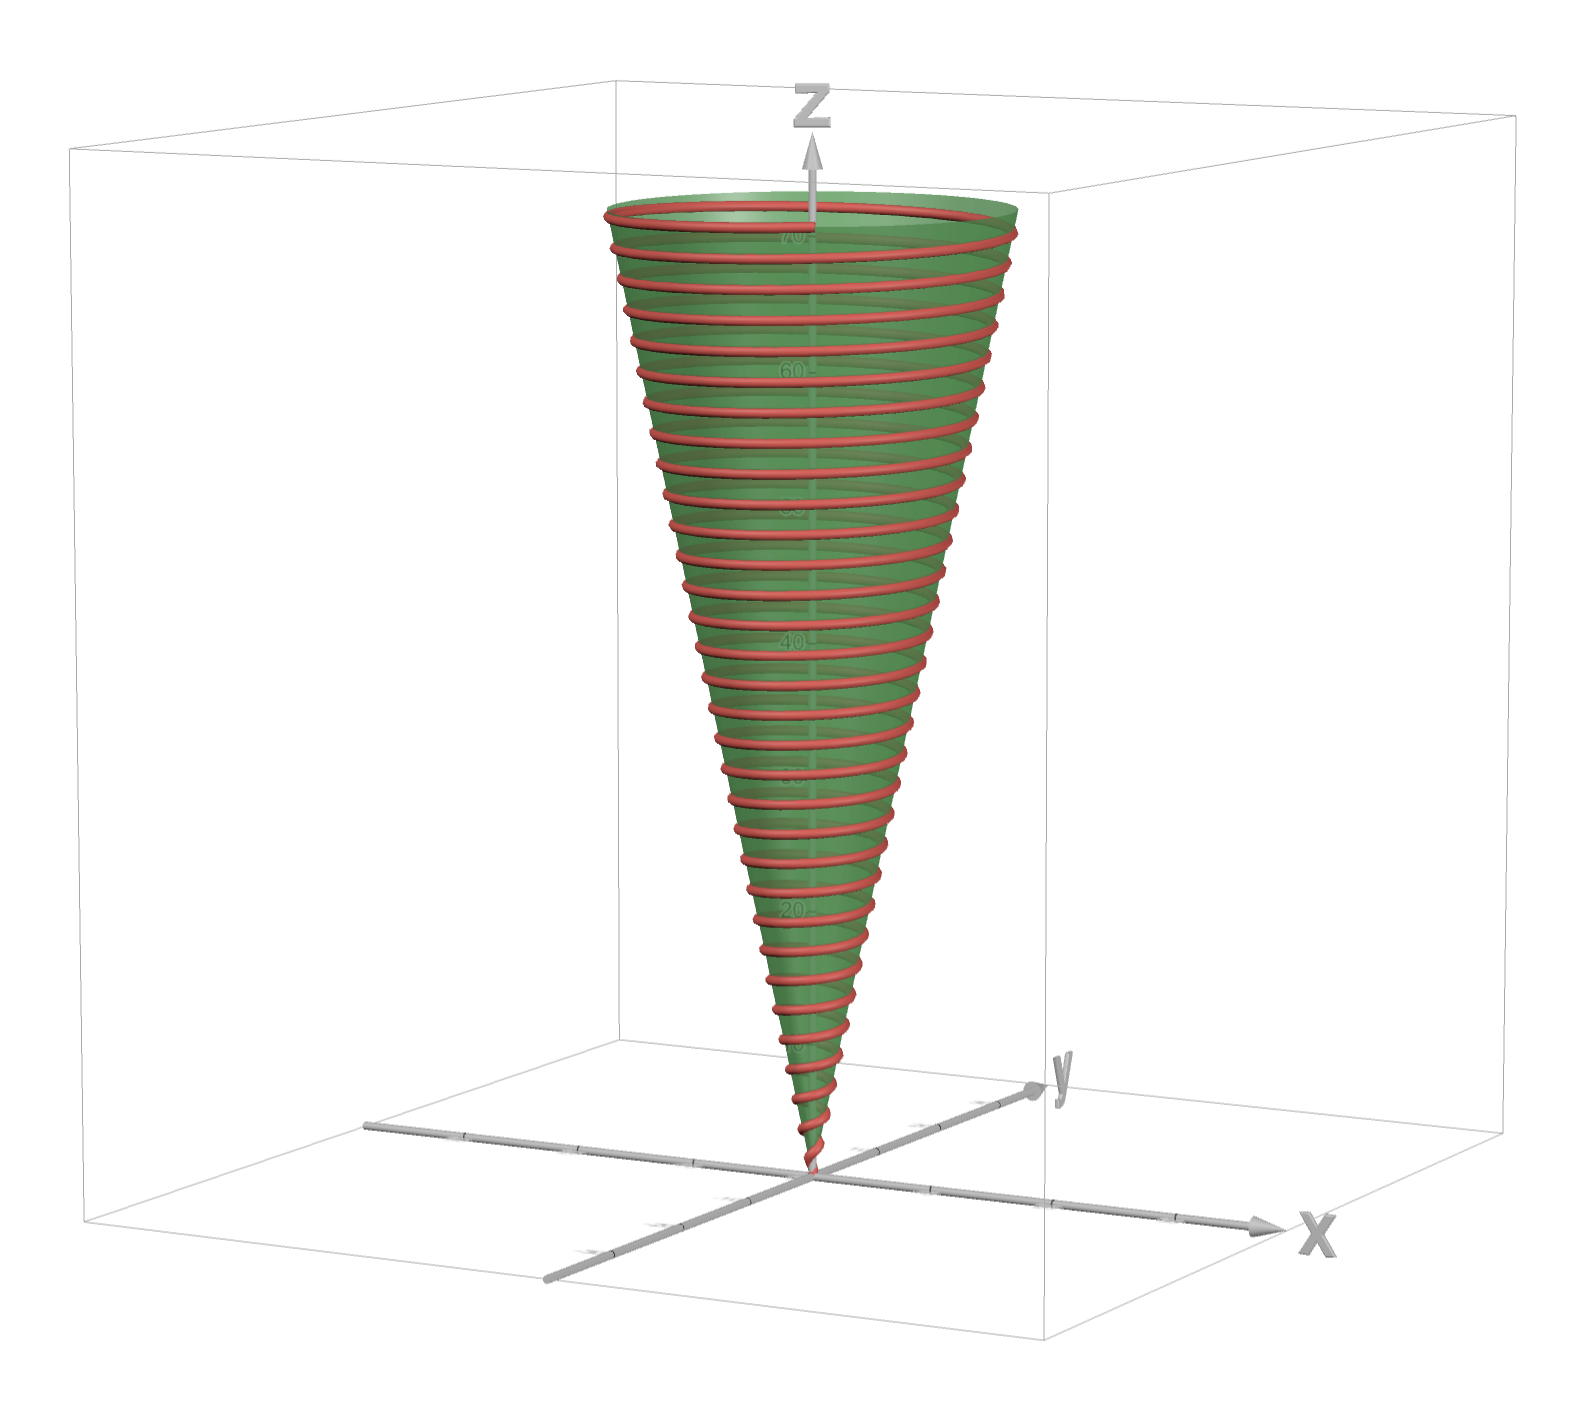
\includegraphics[width=\textwidth]{images/a_vs_b/close.png}
        \caption{$a=0.18$, $b=0.864$}
    \end{subfigure}
    \begin{subfigure}[t]{0.32\textwidth}
        \centering
        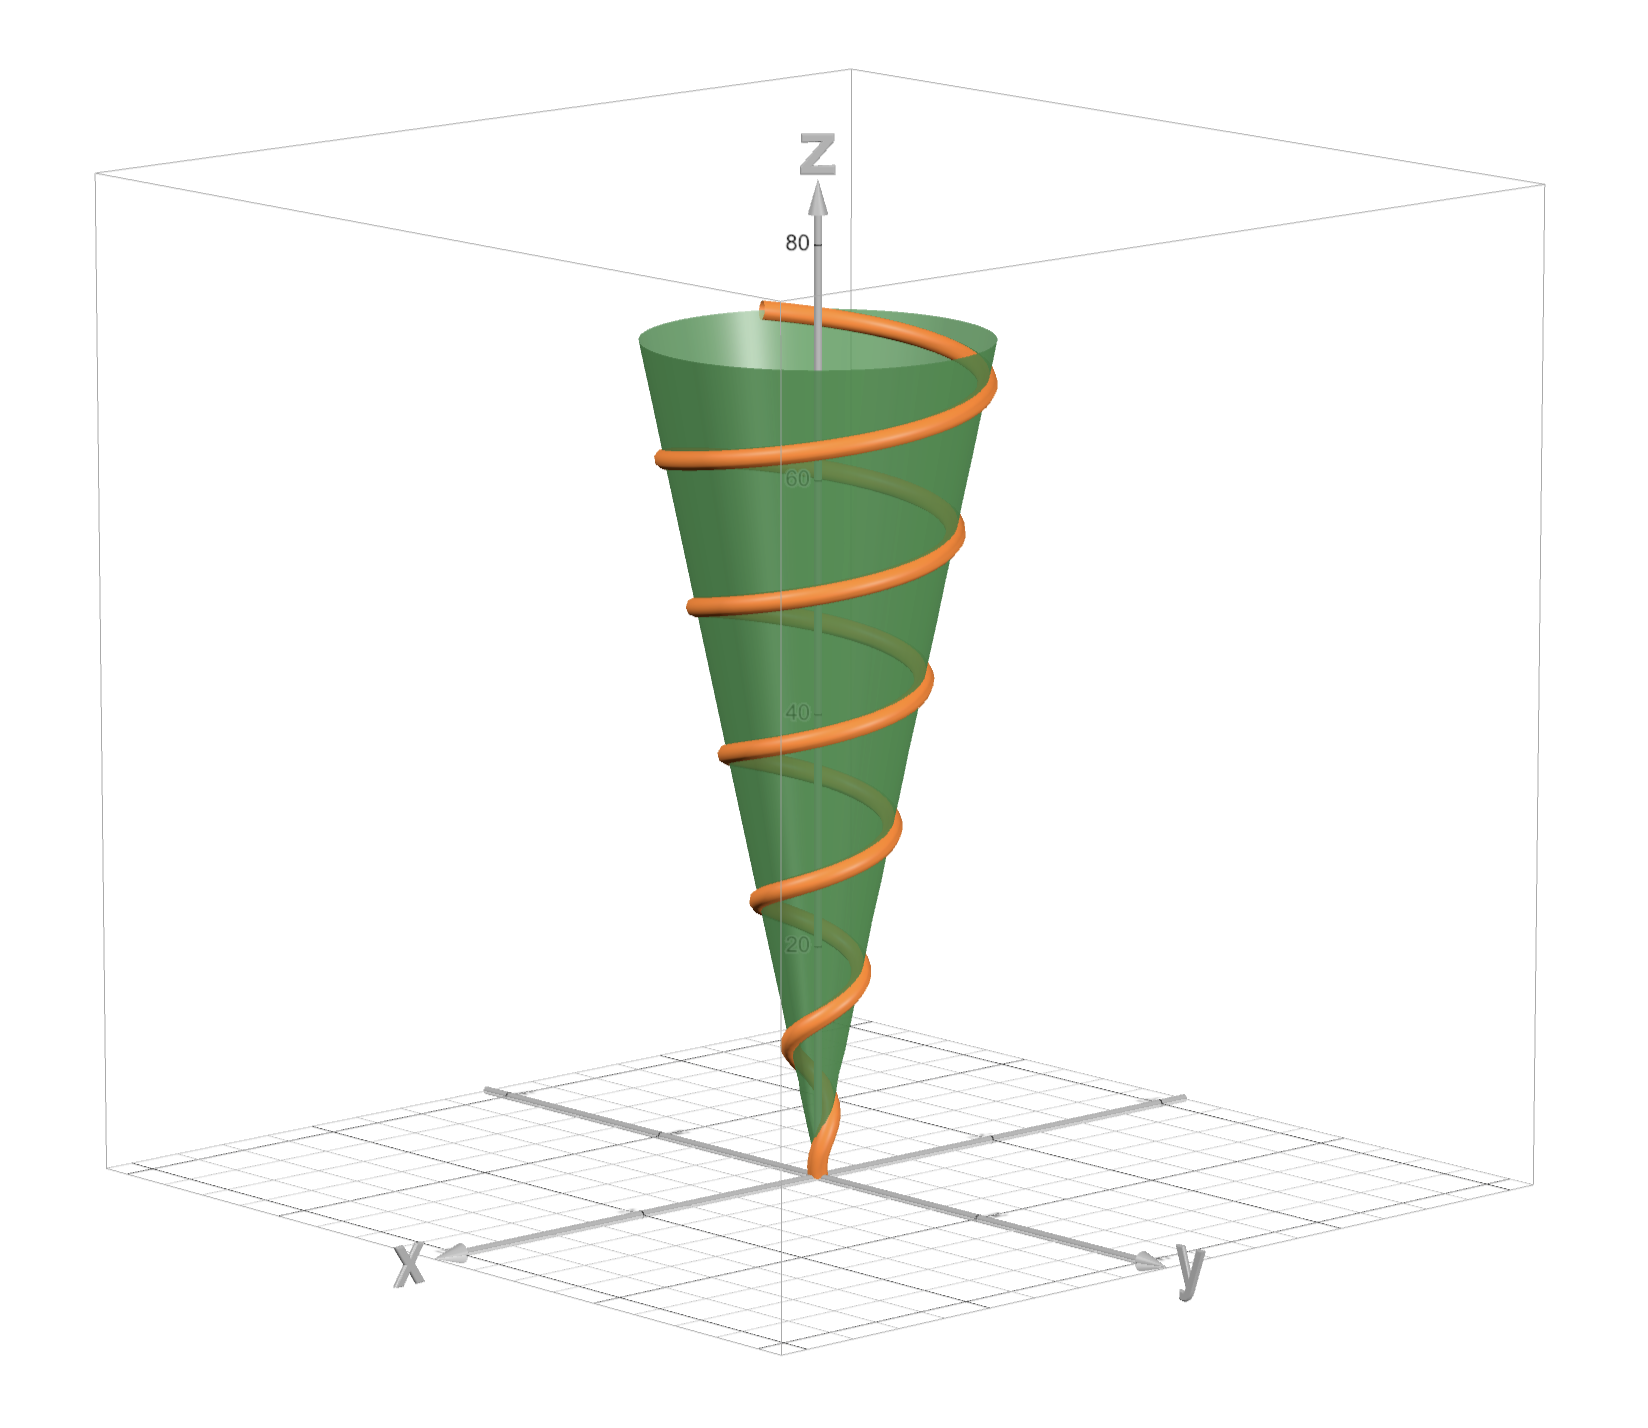
\includegraphics[width=\textwidth]{images/a_vs_b/medium.png}
        \caption{$a=0.42$, $b=2.96$}
    \end{subfigure}
    \begin{subfigure}[t]{0.32\textwidth}
        \centering
        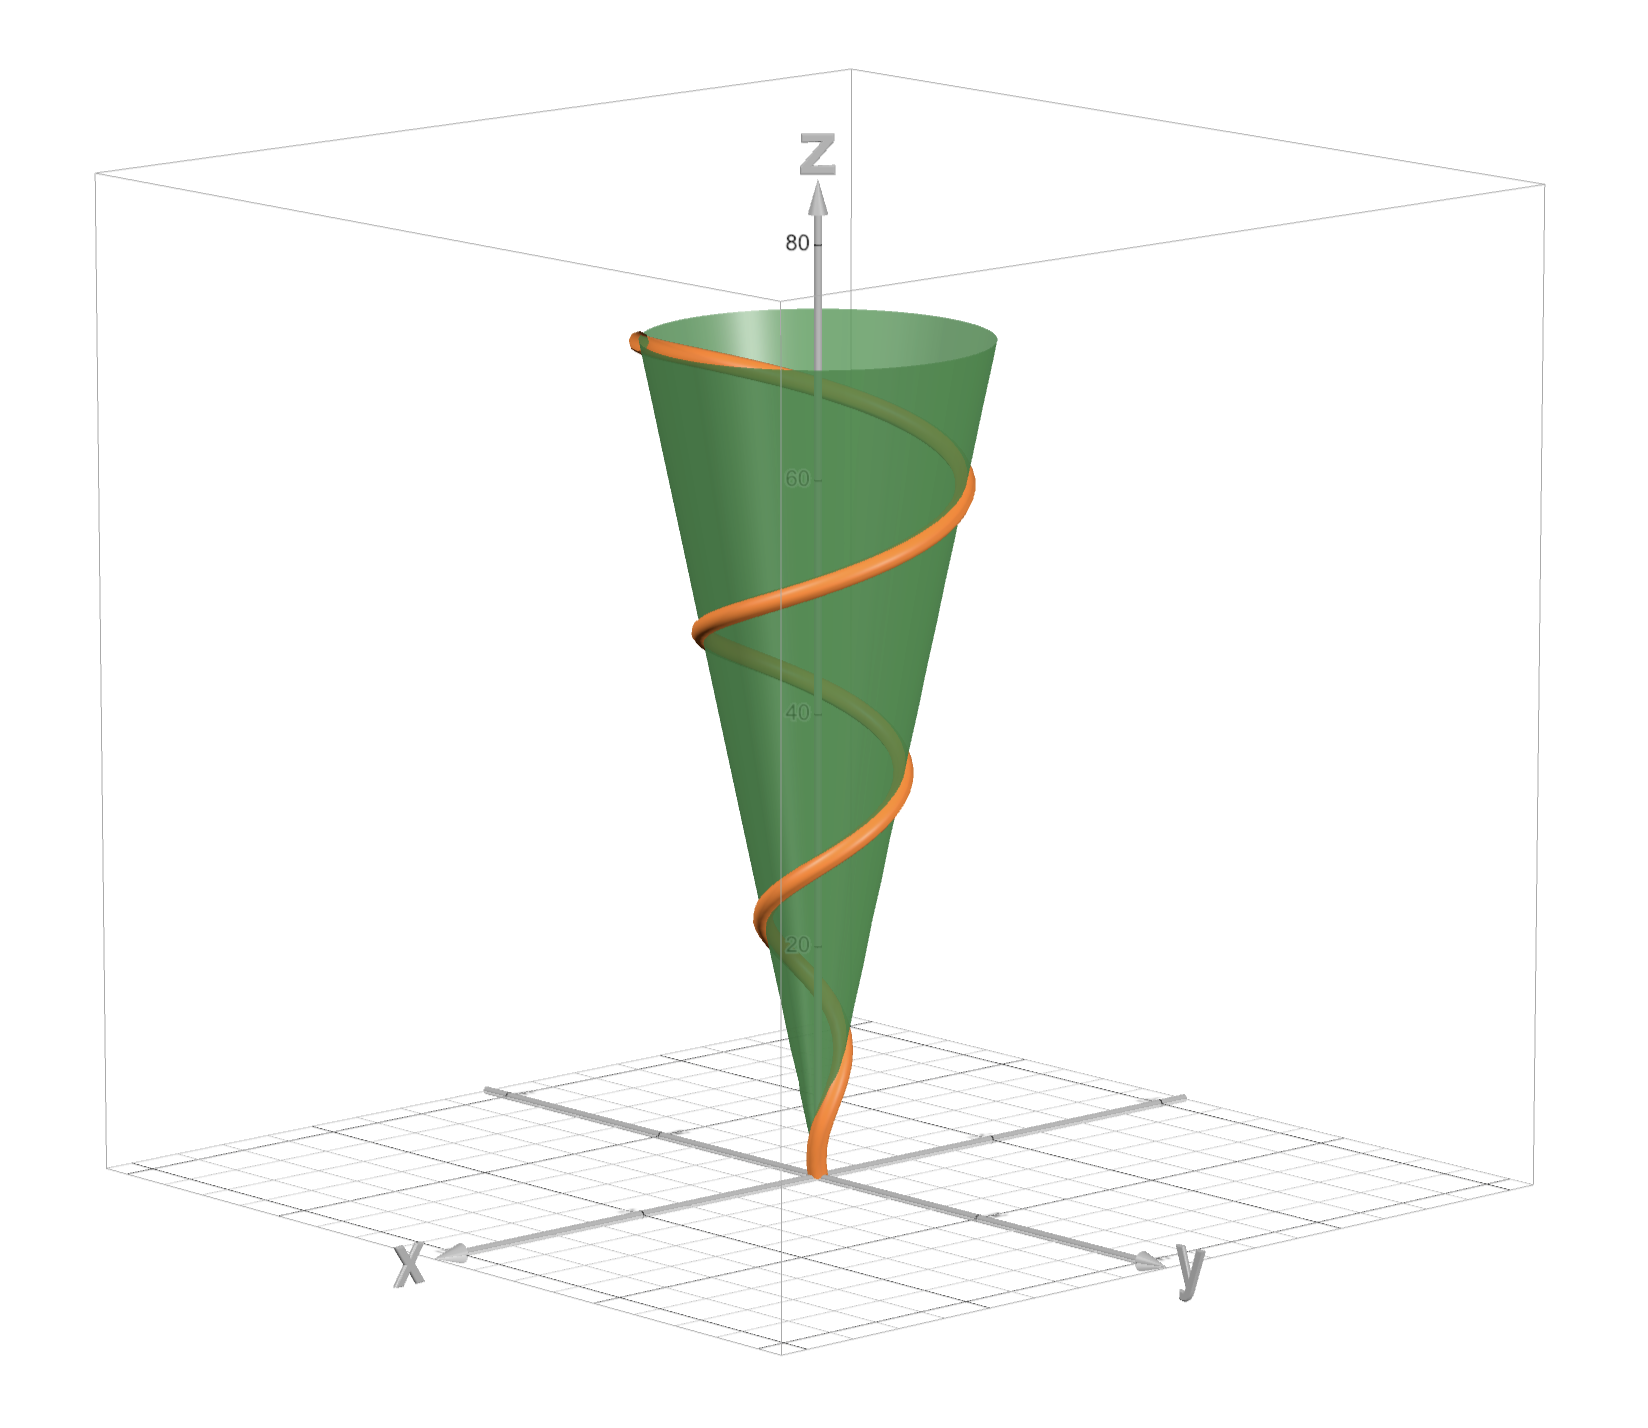
\includegraphics[width=\textwidth]{images/a_vs_b/sparse.png}
        \caption{$a=0.825$, $b=3.96$}
    \end{subfigure}
    \caption{Spirals that have the same ratio of $\frac{a}{b}$ lie on the same cone (generated using \emph{Desmos}).} \label{fig:param_comparison}
\end{figure}

For every rotation of the garland, $t$ increases by $2\pi$ because that is the period of the trigonometric functions sine and cosine. Thus, the change in radial distance, $\Delta \rho$, and change in vertical distance, $\Delta z$, after one full period would be:

\begin{equation*}
    \begin{aligned}[c]
        \Delta \rho & = \rho(t+2\pi) -\rho(t) \\
                    & = a\cdot(t+2\pi) - at   \\
                    & = 2\pi a
    \end{aligned}
    \qquad\qquad\qquad\qquad
    \begin{aligned}[c]
        \Delta z & = z(t+2\pi) -z(t)     \\
                 & = b\cdot(t+2\pi) - bt \\
                 & = 2\pi b
    \end{aligned}
\end{equation*}
In other words, after wrapping around the tree once, the garland has moved outwards by $2\pi a$ and vertically by $2\pi b$. Then, since the distance between successive rotations of the garland is equal to $\lambda$, by the Pythagorean theorem:
\begin{equation}
    \lambda^2 = \Delta \rho^2 + \Delta z^2 =4\pi^2a^2+4\pi^2b^2 \label{eq:spacing}
\end{equation}
From equation \ref{eq:proportion}, $b$ can be isolated to get that $b = \frac{H}{R}a$, which can be substituted back into equation \ref{eq:spacing}:
\begin{equation*}
    \Rightarrow \lambda^2 = 4\pi^2a^2+4\pi^2\cdot\frac{H^2}{R^2} a^2 = 4\pi^2a^2\left(1+\frac{H^2}{R^2} \right)
\end{equation*}
\bulletarrow{Isolating for $a$:}
\begin{equation*}
    a = \sqrt{\frac{\lambda^2}{4\pi^2(1+\frac{H^2}{R^2})}} = \frac{\lambda}{2\pi\sqrt{1+\frac{H^2}{R^2}}} = \frac{\lambda R}{2\pi\sqrt{R^2+H^2}}
\end{equation*}
\bulletarrow{Recognizing that $S=\sqrt{R^2+H^2}$ is the slant height of the cone:}
\begin{equation}
    \Rightarrow a =\frac{\lambda R}{2\pi S}
\end{equation}
\bulletarrow{Plugging this back in equation \ref{eq:proportion}, we get:}
\begin{equation}
    b =\frac{\lambda H}{2\pi S}
\end{equation}
Thus, we finally have that the parametric equation for the garland is:
\begin{equation}
    C(t) = \frac{\lambda}{2\pi S}
    \begin{pmatrix}[0.7]
        Rt\cos{t} \\
        Rt\sin{t} \\
        Ht
    \end{pmatrix}, \quad \forall t \in \left[0, \frac{2\pi S}{\lambda}\right]
\end{equation}
